% Preamble
\documentclass[a4paper, 11pt]{article}
\usepackage[margin=3cm]{geometry}
\usepackage{tikz}
\usepackage{amsmath}
\usepackage{algorithm}
\usepackage{algorithmic}
\usepackage{multicol}
\title{Bioinformatics Assignment}
\author{AMC: Z0132271}
\date{}

% Tree drawing structures
\tikzset{
	solid node/.style={circle, draw, inner sep=2.5, fill=yellow},
	blue node/.style={circle, draw, inner sep=2.5, fill=cyan},
	red node/.style={circle, draw, inner sep=2.5, fill=red},
	green node/.style={circle, draw, inner sep=2.5, fill=green},
}

\tikzset{
	level 1/.style={level distance=30mm, sibling distance=65mm},
	level 2/.style={level distance=30mm, sibling distance=30mm},
	level 3/.style={level distance=30mm, sibling distance=15mm},
	level 4/.style={level distance=30mm, sibling distance=10mm},
  }

% Document
\begin{document}

	\maketitle
	\section{Question 1}
	\subsection{Part A}
	\label{section:1A}
	
	\section{Question 2}
	\subsection{Part A}
	\label{section:2A}
	The algorithm $BUILD$ presented by Aho et al. focuses on the algorithmic goal of reconstructing a tree $T$ that satisfies an input set of constraints $C$. The lowest common ancestor of two nodes $x$ and $y$, denoted $a = LCA(x, y)$, is a node a such that no proper descendant of $a$ (i.e. no node $b$ with $a$ as an ancestor and $b$ is not $a$) which is an ancestor of both $x$ and $y$. This concept is used to formulate constraints for the structure of a tree; the constraint $(i, j) < (k, l)$ over the set of leaves $\{i, j, k, l\}$ specifies that the node $LCA(i, j)$ is a proper descendant of $LCA(k, l)$.
	
	The proposed algorithm implements a recursive process, upon input of a set of nodes $S$ and a set of constraints $C$ (of the aforementioned structure) over these nodes. The base of the recursion is where $S$ only contains a single node; in this case the algorithm outputs the singleton tree $T$ purely consisting of this node as the root. Otherwise, we compute a partition upon the nodes of $S$ with respect to the constraints $C$. A partition $\pi_{C}$ is the subdivision of a set of nodes into subsets $S_{1}, S_{2}, \ldots, S_{r}$ such that the descendants of each child $m$ of the root node of $T$ constitutes the set $S_{m}$. To satisfy $C$, for each constraint $(i, j) < (k, l) \in C$ the corresponding partition $\pi_{C} = S_{1}, \ldots, S_{r}$ must satisfy two conditions. Firstly, both $i$ and $j$ must reside within the same set. Secondly, if $k$ and $l$ lie within the same set, this must imply all nodes $i, j, k$ and $l$ lie within the same set. All sets in the partition must satisfy these conditions; namely, no two nodes may reside within the same set unless specified by either of the prior rules.
	
	For a tree $T$ to exist satisfying $C$, we must be able to find a satisfactory partition $\pi_{C} = S_{1}, \ldots, S_{r}$ where $r \geq 2$---as the existence of at least two subsets to recurse into is a necessary condition when constructing a tree where each non-leaf node has at least two children. Thus, after computing the partition we must check it contains a minimum of two sets; if not, we output a null tree.

	Once a sufficient partition $\pi_{C}$ has been constructed, for each constituent set $S_{m} \in \pi_{C}$ we generate a corresponding subset of constraints $C_{m} \subseteq C$ such that $C_{m}$ contains constraints only involving the nodes of $S_{m}$. We then recurse, implementing the algorithm upon the inputs $S_{m}$ and $C_{m}$ for all $1 \leq m \leq r$. If a tree output by any of these lower recursions is null, the null tree is output at the current level of recursion. Otherwise, on construction of the collection of non-null trees $T_{1}, \ldots, T_{r}$, we output the composite tree $T$ consisting of a new node as the root with $r$ children, where each child node $1 \leq m \leq r$ is the root of the tree $T_{m}$ (with the corresponding full tree expanded below it).
	
	Thus, on conclusion of the highest level of recursion one of two outputs is observed: the tree $T$ with leaves $S$ and a structure satisfying the constraints $C$, or the null tree, indicating no tree exists satisfying the given constraints.

	
	\subsection{Part B}
	\label{section:2B}
	\begin{algorithm}
		\caption{Compute $\pi_{C} = S_{1}, S_{2}, \ldots, S_{r}$}
		\label{alg:partition}
		\textbf{Input:} constraint set $C$ upon node set $S$ \\
		\textbf{Output:} partition $\pi_{C}$
		
		\begin{algorithmic}[1]
			\STATE initialise collection of sets $\pi_{C} \leftarrow \emptyset$
			\IF{$C$ is empty}
				\RETURN $\pi_{C} = $ the collection of singleton sets each containing one node from $S$
			\ELSE
				\FORALL{constraints $(i, j) < (k, l) \in C$}
					\IF{$i$ is in some set $S_{m}$ \algorithmicand\ $j$ is not in any set}
						\STATE allocate $j$ to $S_{m}$
						\STATE add $S_{m}$ to the collection of sets $\pi_{C}$
					\ELSIF{$j$ is in some set $S_{m}$ \algorithmicand\ $i$ is not in any set}
						\STATE allocate $i$ to $S_{m}$
						\STATE add $S_{m}$ to $\pi_{C}$
					\ELSIF{$i$ is in set $S_{m}$ \algorithmicand\ $j$ is in a different set $S_{n}$}
						\STATE merge $S_{m}$ and $S_{n}$ to form a new set $S_{l} = S_{m} \cup S_{n}$ within $\pi_{C}$
					\ELSIF{neither $i$ or $j$ is in any set}
						\STATE create a new set $S_{m} = \{i, j\}$
						\STATE add $S_{m}$ to $\pi_{C}$
					\ENDIF
				\ENDFOR
			
				\FORALL{nodes $n \in S$ which are not in any set}
					\STATE create a new singleton set $S_{m} = \{n\}$
					\STATE add $S_{m}$ to $\pi_{C}$
				\ENDFOR
			
				\FORALL{constraints $(i, j) < (k, l) \in C$}
					\IF{$k$ and $l$ are both in set $S_{m}$ \algorithmicand\ $i$ and $j$ are in a different set $S_{n}$}
						\STATE merge $S_{m}$ and $S_{n}$ to form a new set $S_{l} = S_{m} \cup S_{n}$ within $\pi_{C}$
					\ENDIF
				\ENDFOR
				\RETURN $\pi_{C} = $ the collection of all remaining sets
			\ENDIF
	\end{algorithmic}
	\end{algorithm}
	
	\subsection{Part C}
	\label{section:2C}
	
	% insert Fig A
	\begin{figure}
	\caption{Step 1}
	\label{fig:tree1}
	\begin{center}
	\begin{tikzpicture}[scale=0.6, every node/.style={scale=0.6}]
 
              \node[solid node, label=above:{$S_{1}$}]{}
                child{node[solid node, label=left:{$S_{2}$}]{}
                  edge from parent node{}
                }
                child{node[solid node, label=left:{$S_{3}$}]{}
                  edge from parent node{}
                }
                child{node[solid node, label=right:{$S_{4}$}]{}
                  edge from parent node{}
                }
              ;
            
          \end{tikzpicture}
          \end{center}
          \end{figure}
	
	% insert Fig B
	\begin{figure}
	\caption{Step 2}
	\label{fig:tree2}
	\begin{center}
	\begin{tikzpicture}[scale=0.6, every node/.style={scale=0.6}]
 
              \node[solid node, label=above:{$S_{1}$}]{}
                child{node[solid node, label=left:{$S_{2}$}]{}
                  child{node(l1)[blue node, label=left:{$S_{5}$}]{}
                    child{node[blue node, label=left:{$S_{8}$}]{}
                      child{node[blue node, label=below:{$\mathbf{c}$}, label=left:{$S_{10}$}]{}
                        edge from parent node{}}
                      child{node[blue node, label=below:{$\mathbf{h}$}, label=right:{$S_{11}$}]{}
                        edge from parent node{}}
                      edge from parent node{}}
                    child{node[blue node, label=below:{$\mathbf{a}$}, label=left:{$S_{9}$}]{}
                      edge from parent node{}}
                    edge from parent node{}
                  }
                  child{node(l2)[blue node, label=left:{$S_{6}$}]{}
                    edge from parent node{}
                  }
                  child{node(l3)[blue node, label=left:{$S_{7}$}]{}
                    edge from parent node{}
                  }
                  edge from parent node{}
                }
                child{node[solid node, label=left:{$S_{3}$}]{}
                  edge from parent node{}
                }
                child{node[solid node, label=right:{$S_{4}$}]{}
                  edge from parent node{}
                }
              ;
            
          \end{tikzpicture}
          \end{center}
          \end{figure}
	
	% insert Fig C
	\begin{figure}
	\caption{Step 3}
	\label{fig:tree3}
	\begin{center}
	\begin{tikzpicture}[scale=0.6, every node/.style={scale=0.6}]
 
              \node[solid node, label=above:{$S_{1}$}]{}
                child{node[solid node, label=left:{$S_{2}$}]{}
                  child{node(l1)[blue node, label=left:{$S_{5}$}]{}
                    child{node[blue node, label=left:{$S_{8}$}]{}
                      child{node[blue node, label=below:{$\mathbf{c}$}, label=left:{$S_{10}$}]{}
                        edge from parent node{}}
                      child{node[blue node, label=below:{$\mathbf{h}$}, label=right:{$S_{11}$}]{}
                        edge from parent node{}}
                      edge from parent node{}}
                    child{node[blue node, label=below:{$\mathbf{a}$}, label=left:{$S_{9}$}]{}
                      edge from parent node{}}
                    edge from parent node{}
                  }
                  child{node(l2)[blue node, label=left:{$S_{6}$}]{}
                    child{node[red node, label=left:{$S_{12}$}]{}
                      child{node[red node, label=below:{$\mathbf{j}$}, label=left:{$S_{14}$}]{}
                        edge from parent node{}}
                      child{node[red node, label=below:{$\mathbf{n}$}, label=right:{$S_{15}$}]{}
                        edge from parent node{}}
                      edge from parent node{}}
                    child{node[red node, label=below:{$\mathbf{l}$}, label=left:{$S_{13}$}]{}
                      edge from parent node{}}
                    edge from parent node{}
                  }
                  child{node(l3)[blue node, label=left:{$S_{7}$}]{}
                    child{node[red node, label=below:{$\mathbf{e}$}, label=left:{$S_{16}$}]{}
                      edge from parent node{}}
                    child{node[red node, label=below:{$\mathbf{f}$}, label=left:{$S_{17}$}]{}
                      edge from parent node{}}
                    edge from parent node{}
                  }
                  edge from parent node{}
                }
                child{node[solid node, label=left:{$S_{3}$}]{}
                  edge from parent node{}
                }
                child{node[solid node, label=right:{$S_{4}$}]{}
                  edge from parent node{}
                }
              ;
            
          \end{tikzpicture}
          \end{center}
          \end{figure}
          
	% insert Fig D
	\begin{figure}
	\caption{Step 4---full tree}
	\label{fig:tree4}
	\begin{center}
	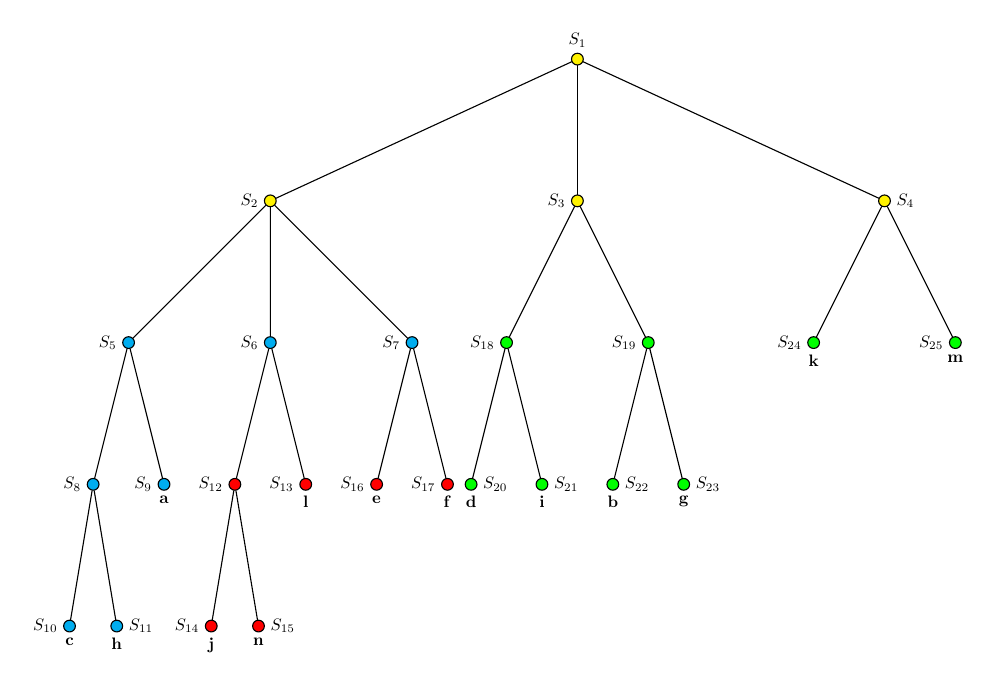
\begin{tikzpicture}[scale=0.6, every node/.style={scale=0.6}]
 
              \node[solid node, label=above:{$S_{1}$}]{}
                child{node[solid node, label=left:{$S_{2}$}]{}
                  child{node(l1)[blue node, label=left:{$S_{5}$}]{}
                    child{node[blue node, label=left:{$S_{8}$}]{}
                      child{node[blue node, label=below:{$\mathbf{c}$}, label=left:{$S_{10}$}]{}
                        edge from parent node{}}
                      child{node[blue node, label=below:{$\mathbf{h}$}, label=right:{$S_{11}$}]{}
                        edge from parent node{}}
                      edge from parent node{}}
                    child{node[blue node, label=below:{$\mathbf{a}$}, label=left:{$S_{9}$}]{}
                      edge from parent node{}}
                    edge from parent node{}
                  }
                  child{node(l2)[blue node, label=left:{$S_{6}$}]{}
                    child{node[red node, label=left:{$S_{12}$}]{}
                      child{node[red node, label=below:{$\mathbf{j}$}, label=left:{$S_{14}$}]{}
                        edge from parent node{}}
                      child{node[red node, label=below:{$\mathbf{n}$}, label=right:{$S_{15}$}]{}
                        edge from parent node{}}
                      edge from parent node{}}
                    child{node[red node, label=below:{$\mathbf{l}$}, label=left:{$S_{13}$}]{}
                      edge from parent node{}}
                    edge from parent node{}
                  }
                  child{node(l3)[blue node, label=left:{$S_{7}$}]{}
                    child{node[red node, label=below:{$\mathbf{e}$}, label=left:{$S_{16}$}]{}
                      edge from parent node{}}
                    child{node[red node, label=below:{$\mathbf{f}$}, label=left:{$S_{17}$}]{}
                      edge from parent node{}}
                    edge from parent node{}
                  }
                  edge from parent node{}
                }
                child{node[solid node, label=left:{$S_{3}$}]{}
                  child{node(l1)[green node, label=left:{$S_{18}$}]{}
                    child{node[green node, label=below:{$\mathbf{d}$}, label=right:{$S_{20}$}]{}
                      edge from parent node{}}
                    child{node[green node, label=below:{$\mathbf{i}$}, label=right:{$S_{21}$}]{}
                      edge from parent node{}}
                    edge from parent node{}
                  }
                  child{node(l2)[green node, label=left:{$S_{19}$}]{}
                    child{node[green node, label=below:{$\mathbf{b}$}, label=right:{$S_{22}$}]{}
                      edge from parent node{}}
                    child{node[green node, label=below:{$\mathbf{g}$}, label=right:{$S_{23}$}]{}
                      edge from parent node{}}
                    edge from parent node{}
                  }
                  edge from parent node{}
                }
                child{node[solid node, label=right:{$S_{4}$}]{}
                  child{node(r1)[green node, label=below:{$\mathbf{k}$}, label=left:{$S_{24}$}]{}
                    edge from parent node{}
                  }
                  child{node(r2)[green node, label=below:{$\mathbf{m}$}, label=left:{$S_{25}$}]{}
                    edge from parent node{}
                  }
                  edge from parent node{}
                }
              ;
            
          \end{tikzpicture}
          \end{center}
          \end{figure}
          
         % Written explanation
	Firstly, we shall label each constraint such that they can subsequently be referred to by index only:
	
	\begin{multicols}{4}
		\begin{enumerate}
			\item $(e, f) < (k, d)$
			\item $(c, h) < (a, n)$
			\item $(j, n) < (j, l)$
			\item $(c, a) < (f, h)$
			\item $(j, l) < (e, n)$
			\item $(n, l) < (a, f)$
			\item $(d, i) < (k, n)$
			\item $(d, i) < (g, i)$
			\item $(c, l) < (g, k)$
			\item $(g, b) < (g, i)$
			\item $(g, i) < (d, m)$
			\item $(c, h) < (c, a)$
			\item $(e, f) < (h, l)$
			\item $(j, l) < (j, a)$
			\item $(k, m) < (e, i)$
			\item $(j, n) < (j, f)$
		\end{enumerate}
	\end{multicols}
	
	The initial inputs into the top layer of recursion are the set of nodes $S = \{a, b, \ldots, n\}$ and the set of constraints $C = \{1, 2, \ldots, 16\}$ (as indexed above). We will refer to these as $S_{1}$ and $C_{1}$.
	
	The first partition we compute is $\pi_{C_{1}}$. Following the fist condition outlined in \ref{section:2A} (and detailed in lines 5--18 in \ref{section:2B}), we generate the initial partition sets $\pi_{C_{1}} = \{e, f\}, \{c, h, a, j, n, l\}, \{d, i, g, b\}, \{k, m\}$. The second condition (algorithm lines 23--26) means we must compute mergers, resulting in the partition $\pi_{C_{1}} = \{a, c, e, f, h, j, l, n\}, \{b, d, g, i\}, \{k, m\}$. We will denote these subsets $S_{2}, S_{3}$, and $S_{4}$. This process is shown through the yellow nodes in Figure \ref{fig:tree1}.
	
	Now we recurse into the subset $S_{2} = \{a, c, e, f, h, j, l, n\}$ with the corresponding constraints subset $C_{2} = \{2, 3, 4, 5, 6, 12, 13, 14, 16\}$ through applying $BUILD(S_{2}, C_{2})$. This recursive step produces the partition $\pi_{C_{2}} = \{a, c, h\}, \{j, l, n\}, \{e, f\}$. We will denote these as $S_{5}, S_{6}$, and $S_{7}$. Next we recurse further into $S_{5} = \{a, c, h\}$ with $C_{5} = \{12\}$. This generates the partition $\pi_{C_{5}} = \{c, h\}, \{a\} = S_{8}, S_{9}$. When recursing into $S_{8}$ we find $C_{8} = \emptyset$ and so output the partition $\pi_{C_{8}} = \{c\}, \{h\} = S_{10}, S_{11}$, thus meaning the nodes $c$ and $h$ are the leftmost deepest leaves. We can also see that $S_{9}$ is a singleton set, and is thus the leaf node $a$ at the above level of recursion. This is visualised through the blue nodes in Figure \ref{fig:tree2}.
	
	As we go up the levels of recursion, we next need to compute $BUILD(S_{6}, C_{6})$ where $S_{6} = \{j, l, n\}$ and $C_{6} = \{6\}$ to generate the partition $\pi_{C_{6}} = \{j, n\}, \{l\} = S_{12}, S_{13}$. We first recurse into $BUILD(S_{12}, C_{12})$, where $C_{12} = \emptyset$, resulting in two singleton sets $S_{14}$ and $S_{15}$ indicating $j$ and $n$ are leaves at this level. On observation of the singleton set $S_{13}$ at the level above we find that $l$ is a leaf here. The next lowest recursion, $BUILD(S_{7} = \{e, f\}, C_{7} = \emptyset)$, gives the singleton sets $S_{16} = \{e\}$ and $S_{17} = \{f\}$, indicating $e$ and $f$ are leaves at this level. Figure \ref{fig:tree3} demonstrates this process through the red nodes.
	
	Next we recurse all the way back to the top level to explore $BUILD(S_{3} = \{b, d, g, i\}, C_{3} = \{8, 10\})$, generating the partition $\pi_{C_{3}} = \{d, i\}, \{b, g\} = S_{18}, S_{19}$. Recursing into $BUILD(S_{18}, C_{18} = \emptyset)$ gives the partition $\pi_{C_{18}} = \{d\}, \{i\} = S_{20}, S_{21}$ and thus leaves $d$ and $i$ at this level. Similarly, $BUILD(S_{19}, C_{19} = \emptyset)$ gives $\pi_{C_{19}} = \{b\}, \{g\} = S_{22}, S_{23}$ and leaves $b$ and $g$. Once again, we return to the top level of recursion and compute $BUILD(S_{4} = \{k, m\}, C_{4} = \emptyset)$, giving the partition $\pi_{C_{C_{4}}} = \{k\}, \{m\} = S_{24}, S_{25}$, which when we recurse into give the final two leaves $k$ and $m$. This concluding part of the algorithm, and the consequentially generated full tree, is shown through in Figure \ref{fig:tree4} (the green nodes indicating the additions from this part).
	
	\subsection{Part D}
	\label{section:2D}
	
	\begin{algorithm}
		\caption{Reverse-BUILD}
		\label{alg:reverse}
		\textbf{Input:} tree $T$ with labelled leaves $S$ \\
		\textbf{Output:} a corresponding the set of constraints $C$
		
		\begin{algorithmic}[1]
			\STATE initialise $C \leftarrow \emptyset$
			
			\FORALL{non-root layers $L_{i}$ of $T$ (from deepest leaves to the layer before the root)}
				
				\STATE assign each leaf $l$ at layer $L_{i}$ the singleton set containing its value $S_{l} = \{v_{l}\}$
				
				\FORALL{non-leaf nodes $p$ in layer $L_{i + 1}$ (above $L_{i}$)}
					
					\STATE form the partition $\pi_{p} = S_{1}, S_{2}, \ldots, S_{N}$ consisting of the sets assigned to each of the $N$ children of $p$
					
					\FORALL{sets $S_{m} \in \pi_{p}$ containing more than one element}
						
						\FORALL{other sets $S_{n} \in \pi_{p} \setminus S_{m}$}
							
							\IF{no constraint $(a, b) < (c, d) \in C$ exists where $a, b \in S_{m}$ and either $c \in S_{n}$ or $d \in S_{n}$}
								\STATE sample two distinct leaves from the first set $a, b \in S_{m}$
								\STATE set $c$ equal to either of these leaves $a$ or $b$
								\STATE sample another leaf from the second set set $d \in S_{n}$
								\STATE add a new constraint over these values: $C \leftarrow (a, b) < (c, d)$
							\ENDIF
							
						\ENDFOR
						
						\STATE merge the sets of $\pi_{p}$ and assign this to the corresponding parent node $p$
					\ENDFOR
				\ENDFOR
			\ENDFOR
			\RETURN the set of constraints $C$
	\end{algorithmic}
	\end{algorithm}
	
	The proposed algorithm \emph{Reverse-BUILD} in Algorithm \ref{alg:reverse} implements an iterative method for building a set of constrains $C$ from a given tree $T$ through which we could apply the $BUILD$ algorithm and construct a tree isomorphic to $T$. It relies upon splitting $T$ into distinct layers, where each layer contains all nodes at the sample depth, and considering each of these layers $L_{i}$ through a bottom-up approach. We start at the deepest layer and assign each of the leaves its own singleton set; sets on sibling leaves are then merged and assigned to label the corresponding parent node $p$.
	
	We then consider the next layer, where similarly any leaves are assigned to singleton sets. Next, sibling nodes in layer $L_{i}$ with the same parent $p$ in layer $L_{i + 1}$ are grouped. Each of these groups corresponds to a partition; namely, for the parent node $p$ in layer $L_{i + 1}$ with $N$ children in layer $L_{i}$, a partition is constructed of the sets associated with each of these children: $\pi_{p} = S_{1}, S_{2}, \dots, S_{N}$. For each of the constituent sets $S_{m} \in \pi_{p}$, we then cycle through all other sets $S_{n}$ in the same partition and ensure there is a constraint which links the elements of $S_{m}$ and $S_{n}$ in line with the satisfaction of the two rules outlined in Section \ref{section:2A}.
	
	The construction of this constraint (in absence of one existing already) is implemented through the lines 8--13 in Algorithm \ref{alg:reverse}. We need to ensure this is the case between every set (i.e. the rules are followed exactly) in the partition such that the correct dependencies between nodes are exhibited in the full constraint set. If this is followed, it maintains that when the $BUILD$ algorithm is applied to the full set we can once again generate the same partitions (when we reach this level of the tree).
		
\end{document}
